\documentclass{beamer}
\usecolortheme[named=brown]{structure}
\usetheme{Malmoe}
\usepackage{natbib}
\usepackage{graphicx}

\author{James Church}
\title{A Gentle Introduction to R}

\begin{document}

\frame[plain]{ \titlepage }

\begin{frame}{A Gentle Introduction to R}

    Outline

    \begin{itemize}
        \item Why R?
        \item Tools that I'm using in this presentation.
        \item Important Data Types
        \item Random Number Generation
        \item Plotting
        \item File Input
        \item Simple Linear Regression
        \item Multiple Linear Regression
    \end{itemize}

\end{frame}

\begin{frame}{Why R?}
     \begin{itemize}
        \item You wish to analyze.
        \item You wish to create beautiful plots.
    \end{itemize}
\end{frame}

\begin{frame}{Tools Used in this Presentation}
    \begin{itemize}
        \item R
        \item RStudio
    \end{itemize}
\end{frame}

\begin{frame}{Random Number Generation}

    Stupid Math Tricks: Computing Pi using Random Numbers

    First: The Theory

    \begin{itemize}
        \item A square with sides of length 2 has its center at the origin.
        \item A circle with a radius of length 1 has its center at the origin.
        \item The length of the side of the square is 2 times the radius of the circle. 
	\item Area of the square: $(2r)^2$ or $4r^2$ or $4$.
	\item Area of the circle: $\pi r^2$ or $\pi$.
	\item The ratio of the area of the two shapes is

	\begin{math}
	\frac{\pi}{4} = \frac{Area\:of\:the\:Circle}{Area\:of\:the\:Square}
	\end{math}

	\item This means we can write $\pi$ as

	\begin{math}
	\pi = \frac{4 \times Area\:of\:the\:Circle}{Area\:of\:the\:Square}
	\end{math}

    \end{itemize}
\end{frame}

\begin{frame}{Random Number Generation}

    Stupid Math Tricks: Computing Pi using Random Numbers

    Second: The Practice

    \begin{itemize}
        \item Imagine our square is now a dartboard.
	\item We have 1 million darts, all to throw at the dartboard.
	\item All 1 million darts must land in the square.
	\item We count the darts landing in the circle. (Our friend Pythagoras has an old formula for doing this.)
	\item We then compute $\pi$:

	\begin{math}
	\pi = \frac{4 \times Area\:of\:the\:Circle}{Area\:of\:the\:Square} = \frac{4 \times Darts\:in\:the\:Circle}{1 million}
	\end{math}

    \end{itemize}
\end{frame}

\begin{frame}{Random Number Generation}

    Stupid Math Tricks: Computing Pi using Random Numbers

    Third: The Code

    \begin{verbatim}
    > # Start throwing darts
    > n <- 100000
    > x <- runif(n, -1, 1)
    > y <- runif(n, -1, 1)
    > 
    > # Determine which darts are in the circle
    > in.circle <- sqrt(x^2 + y^2)<=1
    > 
    > # Estimate pi and calcualte the error.
    > estimated.pi <- 4 * sum(in.circle) / n
    > estimated.pi
    [1] 3.14512
    > estimated.pi.percent.error <- 100*abs(estimated.pi - pi)/pi
    > estimated.pi.percent.error
    [1] 0.1122789
    \end{verbatim}

\end{frame}

\begin{frame}{Random Number Generation}

    Stupid Math Tricks: Computing Pi using Random Numbers

    Forth: Let's graph this.

    \begin{verbatim}
    > matplot(x[in.circle==T], y[in.circle==T], col='blue');
    > matplot(x[in.circle==F], y[in.circle==F], col='red', add=T)
    \end{verbatim}

    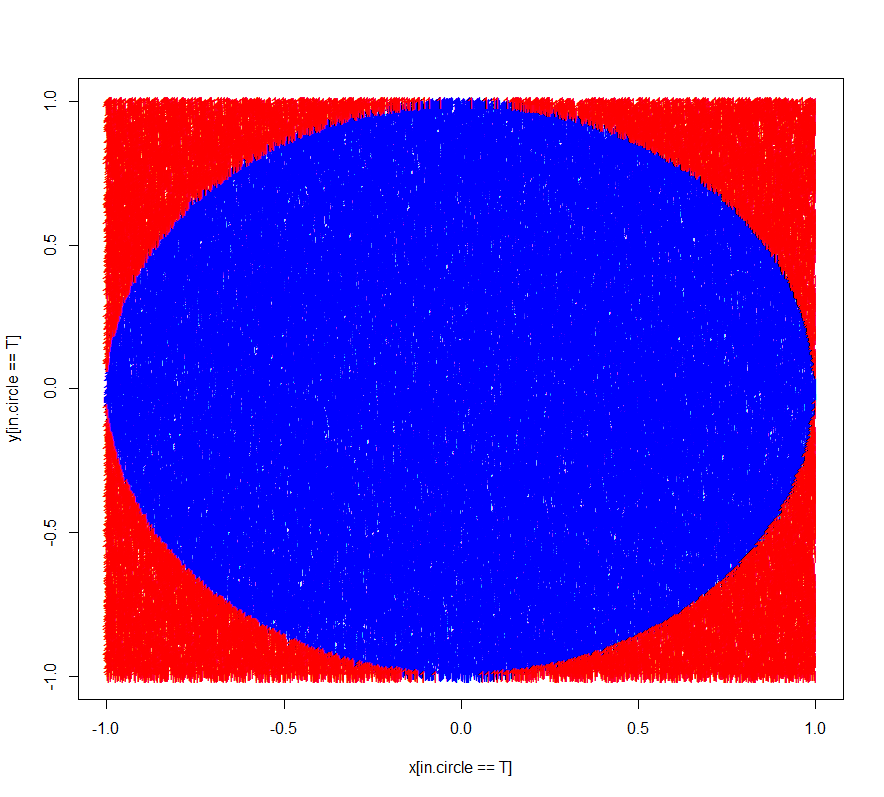
\includegraphics{dartboard.png}

\end{frame}


\end{document}
